\documentclass[11pt,a4paper]{article}
\usepackage[utf8]{inputenc}
\usepackage[francais]{babel}
\usepackage[T1]{fontenc}
\usepackage{amsmath}
\usepackage{amsfonts}
\usepackage{amssymb}
\usepackage{graphicx}

\begin{document}

\title{Rapport de TP de Réseaux II \\ Projet tiny internet}
\author{Clément Tamines, Florent Delgrange}
\maketitle


\section{Introduction}
Le but de ce projet est de modéliser une interconnexion de réseaux. Pour modéliser ces réseaux, nous utiliserons C-BGP. Nous allons tout d'abord configurer les routeurs et les divers domaines auquel ils appartiennent.


Le but de ce projet est de créer une topologie réseau et de configurer différents AS à l'intérieur de celle-ci. Nous allons ensuite configurer le routage intradomaine et les routes statiques. Enfin, nous ajouterons des filtres de routage pour modéliser les différentes relations de "business" entre les domaines participants. Nous décrirons dans ce rapport les techniques utilisées ainsi que la logique derrière nos choix d'implémentation.

\section{Ajout des noeuds}
Nous avons tout d'abord ajouté les différents noeuds de la topologie. Un noeud représente un routeur dans le réseau. Chaque routeur appartient à un domaine spécifique pour lequel nous connaissons le préfixe associé. Nous prendrons donc comme convention d'attribuer les  premières adresses du préfixe correspondantes au numéro du routeur dans le domaine. Le routeur R1 de BigCarrier (qui possède le préfixe 1.0.0.0/8) se verra attribuer l'adresse 1.0.0.1.\\
La commande utilisée pour ajouter un noeud à la topologie est \textbf{net add node 1.0.0.1}.

\section{Ajout des liens entre les routeurs}
Nous allons maintenant ajouter les liens entre les différents routeurs. L'ajout de ces liens se fait d'abord au niveau de la couche physique, nous ajoutons un lien entre deux noeuds via la commande suivante \textbf{net add link 1.0.0.1 1.0.0.2}
\subsection{Liens intradomaine}
Pour le routage intradomaine via iBGP, nous devons décrire la façon dont les routeurs sont reliés dans le domaine et donner des poids à ces liens. Nous utiliserons ici le délai en ms comme poids dans iBGP, le poids minimum étant donc le lien le plus rapide.\\
La commande utilisée pour donner un poids igp entre deux routeurs du même domaine est \textbf{net link 1.0.0.1 1.0.0.2 igp-weight --bidir 1} l'argument bidir nous indique que le poids est le même dans les deux sens.

\subsection{Liens interdomaine}
Afin de relier les routeurs de différents domaines entre eux, il est nécessaire de dire quels préfixes sont atteignables via un certain routeur ainsi qu'un poids pour le lien via des routes statiques. Nous utiliserons comme poids le temps en ms sur le lien. Pour dire que le routeur 1.0.0.1 est lié au routeur 2.0.0.1 et permet d'atteindre le préfixe 2.0.0.1/8 avec un poids de 65, la commande suivante sera utilisée \textbf{net node 1.0.0.1 route add 2.0.0.1/8 -oif=2.0.0.1 65}

\section{Configuration des routeurs}
Afin de configurer les routeurs, plusieurs étapes sont nécessaires. Tout d'abord nous allons devoir annoncer les préfixes associés aux routeurs, plusieurs préfixes étant associés au même domaine. Pour ajouter un routeur à BGP et entrer en mode configuration du routeur : \\ \textbf{bgp add router 11537 3.0.0.3\\
bgp router 3.0.0.3\\
	...\\
	exit}\\
Pour ajouter un routeur dans le même domaine, et activer la connexion entre les deux routeurs, nous utilisons la commande \textbf{add peer 20965 4.0.0.1\\
	peer 4.0.0.1 up}
	
Pour ajouter un routeur pair dans un autre domaine, et activer la connexion ainsi que de prévenir le paire de changer le next hop dans le chemin, nous utiliserons la commande \textbf{add peer 2 2.0.0.1
	peer 2.0.0.1 next-hop-self\\
	peer 2.0.0.1 up}
	
	Pour dire quels préfixes sont annoncés par un routeur, nous utiliserons la commande suivante. Il est important de noter que plusieurs préfixes peuvent être annoncés par un routeur \textbf{bgp router 3.1.0.1 add network 3.1.0.0/16}
	
\section{Filtres de routage}
Afin de décrire les relations de business entre les différents domaines, nous avons créé plusieurs filtres de routage. Les relations commerciales entre les différents domaines sont décrites sur le schéma suivant : \\

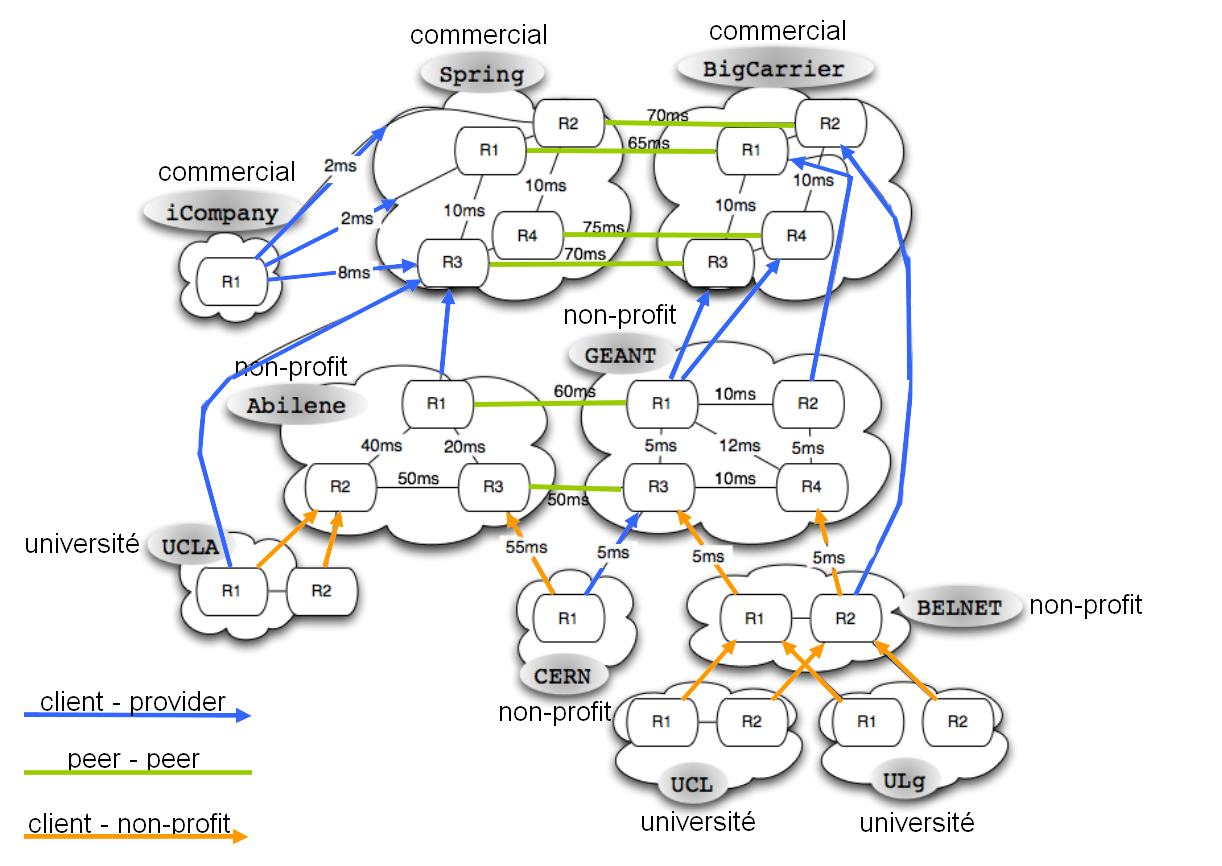
\includegraphics[scale=0.3]{topo.png}
\end{document}